\documentclass{article}
\usepackage[UTF8]{ctex}
\usepackage{pythonhighlight}
\usepackage{markdown}
\usepackage{listings}
\lstset{
    basicstyle          =   \tt,          % 基本代码风格
    identifierstyle=\color{brown!80!black},
    keywordstyle        =   \color{purple}\bfseries,          % 关键字风格
    commentstyle        =   \rmfamily\itshape,  % 注释的风格,斜体
    stringstyle         =   \ttfamily,  % 字符串风格
    flexiblecolumns,                % 别问为什么,加上这个
    numbers             =   left,   % 行号的位置在左边
    showspaces          =   false,  % 是否显示空格,显示了有点乱,所以不现实了
    numberstyle         =   \zihao{-5}\ttfamily,    % 行号的样式,小五号,tt等宽字体
    showstringspaces    =   false,
    captionpos          =   t,      % 这段代码的名字所呈现的位置,t指的是top上面
    frame               =   lrtb,   % 显示边框
    backgroundcolor=\color[RGB]{245,245,244},
}


% Language setting
% Replace `english' with e.g. `spanish' to change the document language
\usepackage[english]{babel}
\usepackage{float}
% Set page size and margins
% Replace `letterpaper' with `a4paper' for UK/EU standard size
\usepackage[letterpaper,top=2cm,bottom=2cm,left=3cm,right=3cm,marginparwidth=1.75cm]{geometry}

% Useful packages
\usepackage{amsmath}
\usepackage{graphicx}
\usepackage[colorlinks=true, allcolors=blue]{hyperref}

\title{普物虚拟实验报告1}
\author{雷远航 \ 学号:3210105807}

\begin{document}

\maketitle

\begin{abstract}
    光栅单色仪
\end{abstract}

\section*{一、实验目的}
\subsubsection*{- 加深光的波动性的理解}
\subsubsection*{- 了解光的衍射原理}
\subsubsection*{- 光谱分析与测量}



\section*{二、实验原理}

\subsection*{1.单缝的夫琅和费衍射:}
光的衍射现象是指光遇到障碍物时偏离直线传播方向的现象。

产生暗纹的条件是:$asin{\theta} = k{\lambda}$

暗条纹的中心位置是:$x = k\frac{s\lambda}{a}$

产生明条纹的条件是:$asin{\theta = (k + \frac{1}{2})\lambda}$

明条纹的中心位置为: $x = (k + \frac{1}{2}) \frac{s\lambda}{a}$

\subsection*{2.单缝衍射的振幅分布公式和光强分布公式:}

$I_{\theta}$ = $I_{0}$$(\frac{sinu}{u})^{2}$

u = $\frac{\pi asin\theta}{\lambda}$
光强分布的图像如下:
    \begin{figure}[H]
    \centering
    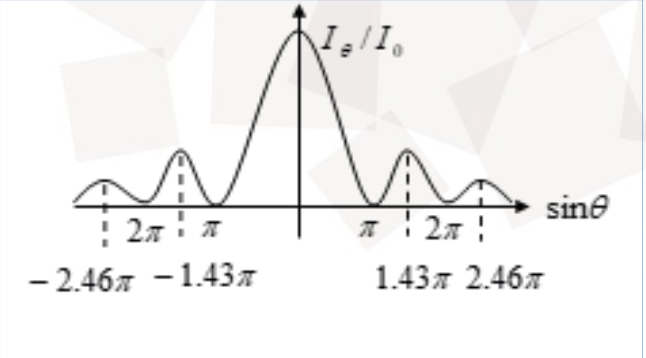
\includegraphics[width=0.5\textwidth]{1.png}
    \end{figure}


\subsection*{3.光栅衍射:}
常用的衍射光栅分透射式与反射式两种。透射式光栅是用金刚石刀在平面透明玻璃板上刻划平行、等间距又等宽的直痕而制成的。反射式光栅是在坚硬的合金板或高反射率平面镜上刻划而成的。

\subsection*{4.光栅方程:}

光栅衍射条纹的光强分布是由各缝引起的光振动相干叠加的结果。

各缝光振动振幅可认为近似相等.对于衍射角为$\theta$的P点,相邻两缝
光振动的相位差为:

$\triangle\phi = \frac{2\pi d sin\theta}{\lambda}$

N个光振动矢量的叠加,求与单缝衍射的光强分布的方程类似,每个光振动构成了
以O为圆心,R为半径的圆等长弦,所对应的圆心角均为$\triangle\phi$,由几何关系
可得合振幅方程:

$A = 2Rsin(\frac{\triangle\phi\cdot N}{2})$

\subsection*{5.氢原子的里德堡常数}

\begin{figure}[H]
    \centering
    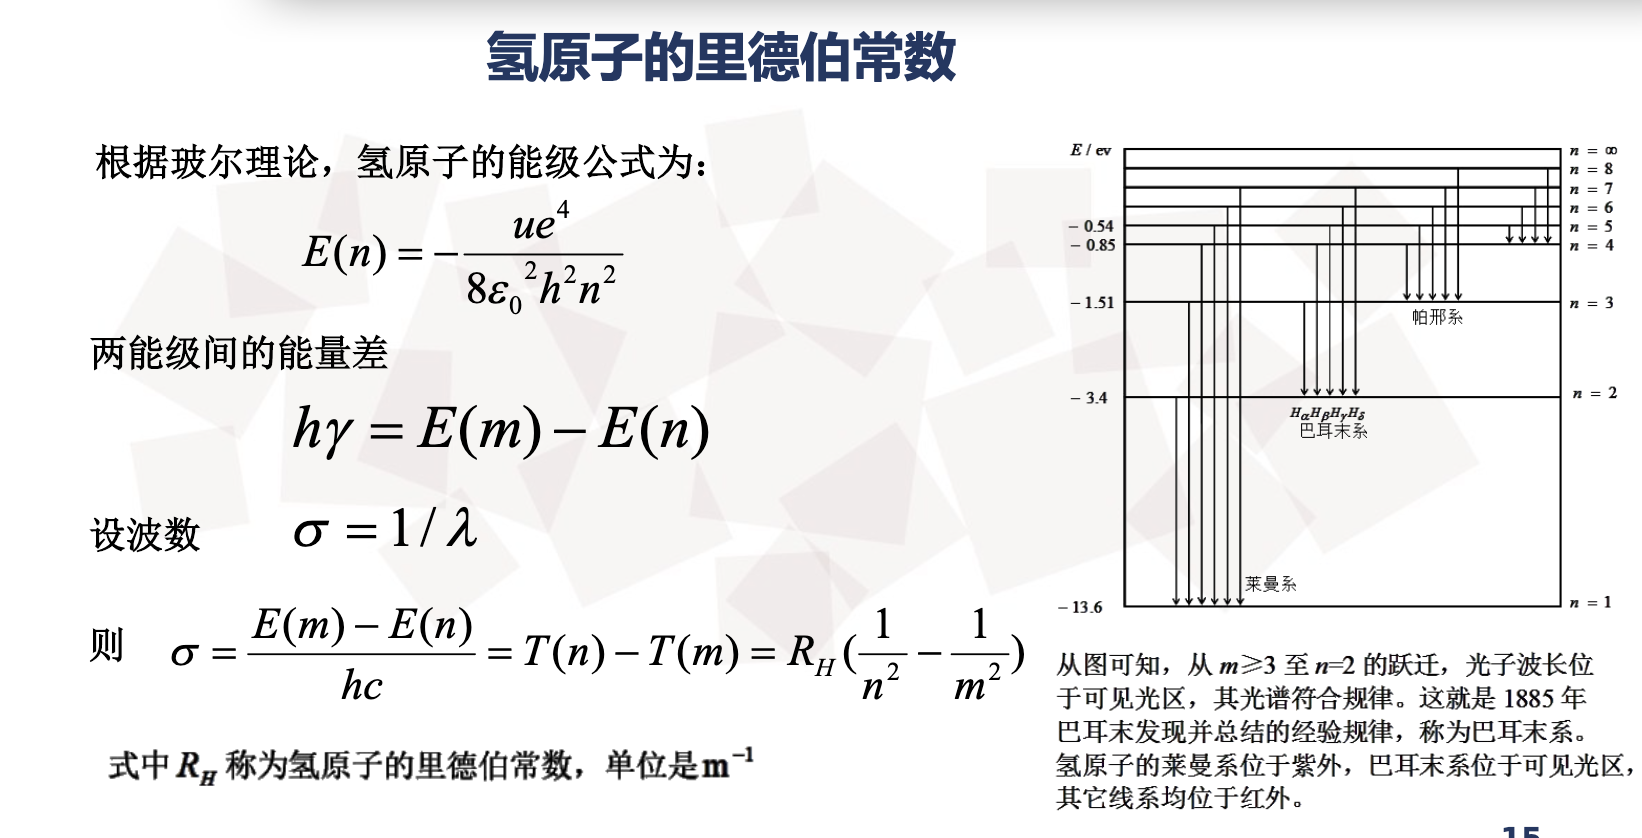
\includegraphics[width=0.7\textwidth]{2.png}
    \end{figure}


\subsection*{6.实验仪器}
\begin{figure}[H]
    \centering
    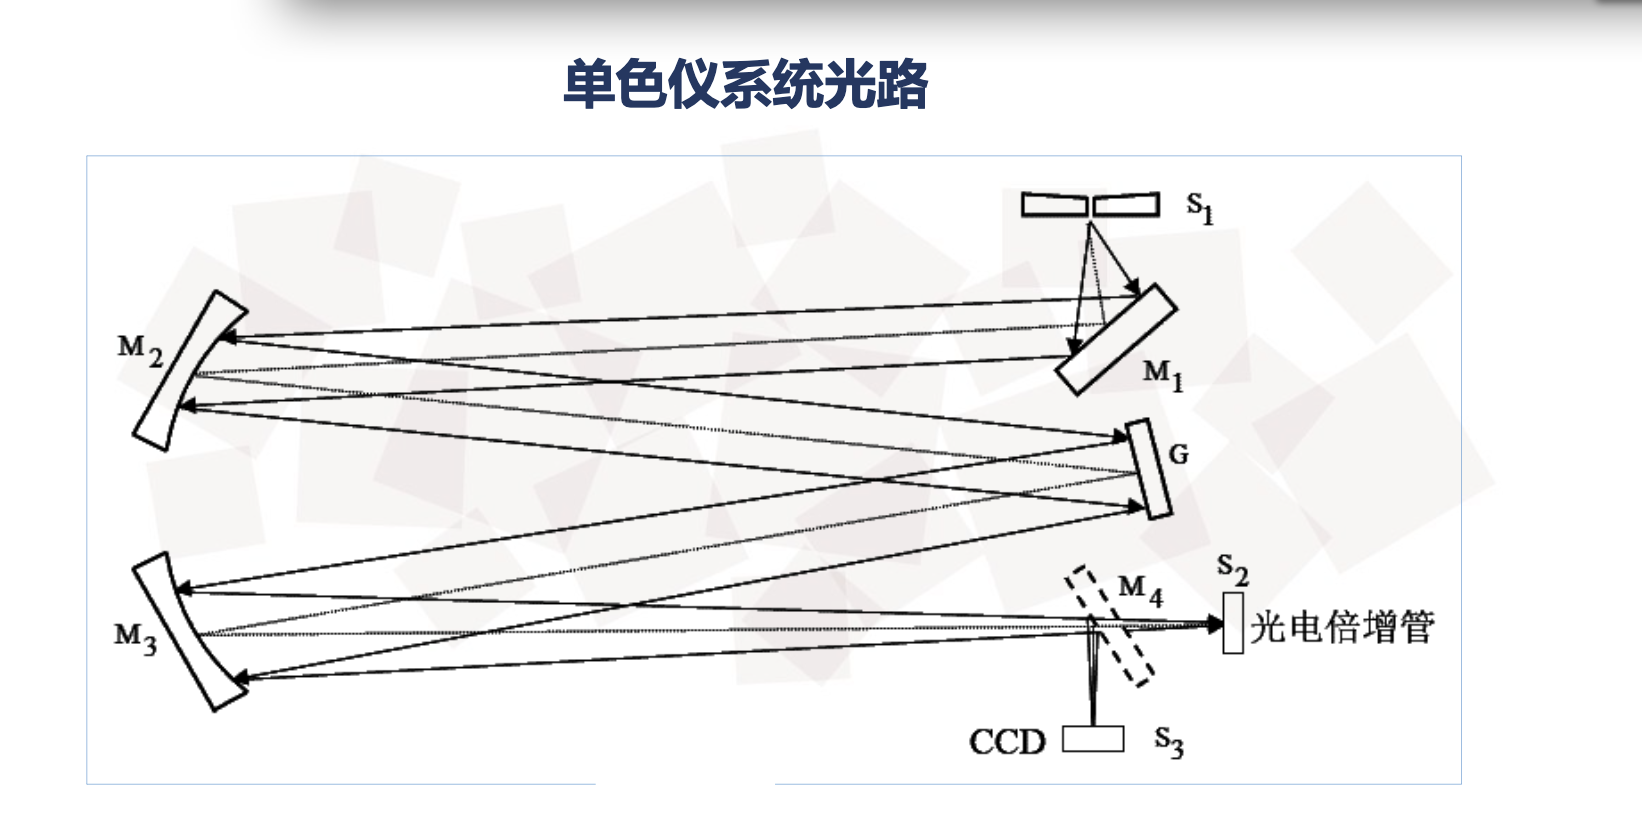
\includegraphics[width=0.7\textwidth]{3.png}
    \end{figure}

    \begin{figure}[H]
        \centering
        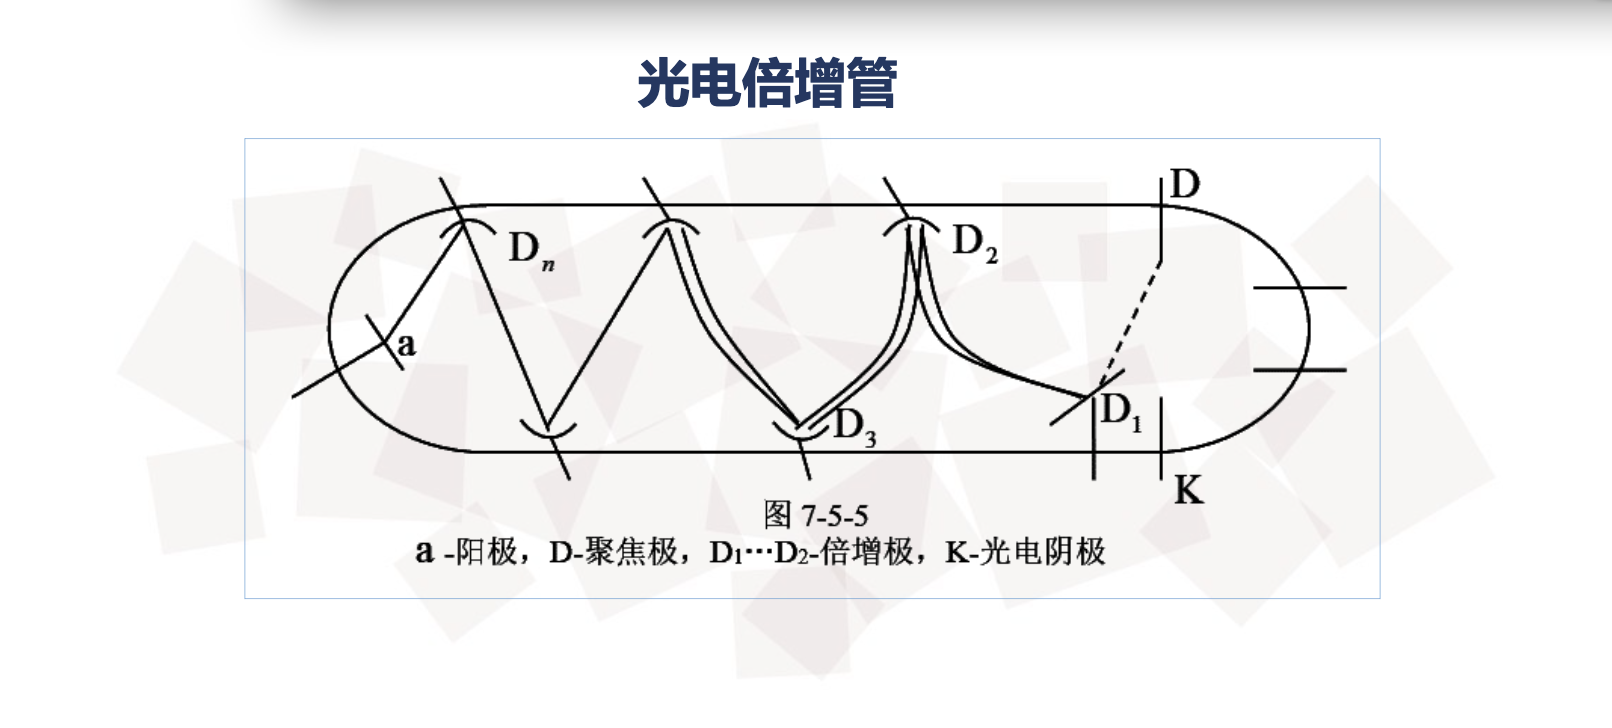
\includegraphics[width=0.7\textwidth]{4.png}
        \end{figure}
    

\section*{三、实验数据}

\subsection*{采样氢光谱线图}

\begin{figure}[H]
    \centering
    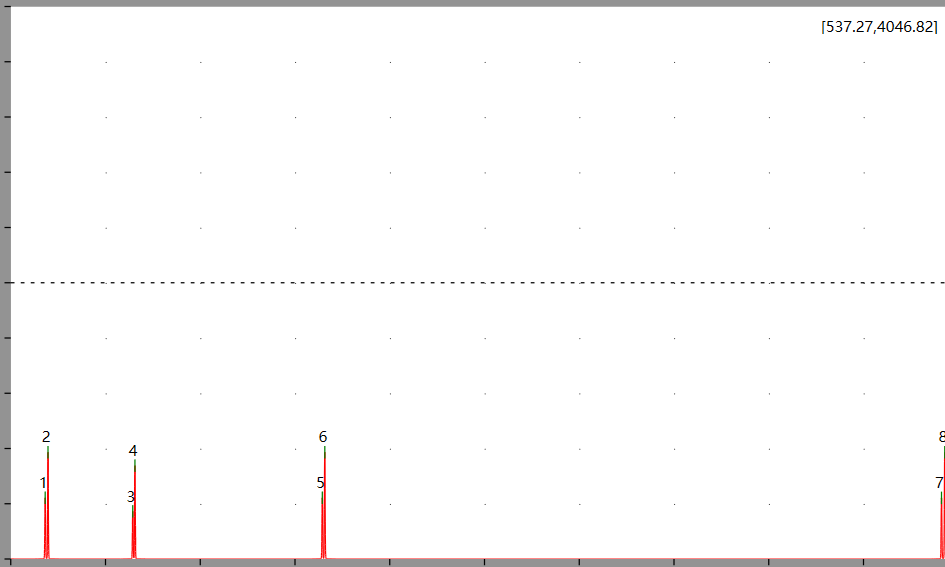
\includegraphics[width=0.7\textwidth]{虚拟1/1.png}
    \caption{\label{Lab12}氢光谱曲线}
    \end{figure}

    \begin{figure}[H]
        \centering
        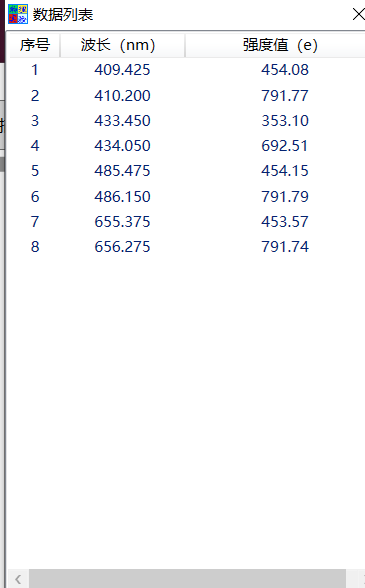
\includegraphics[width=0.5\textwidth]{虚拟1/2.png}
        \caption{\label{Lab12}实验数据}
        \end{figure}

实验数据处理如下:

\begin{figure}[H]
    \centering
    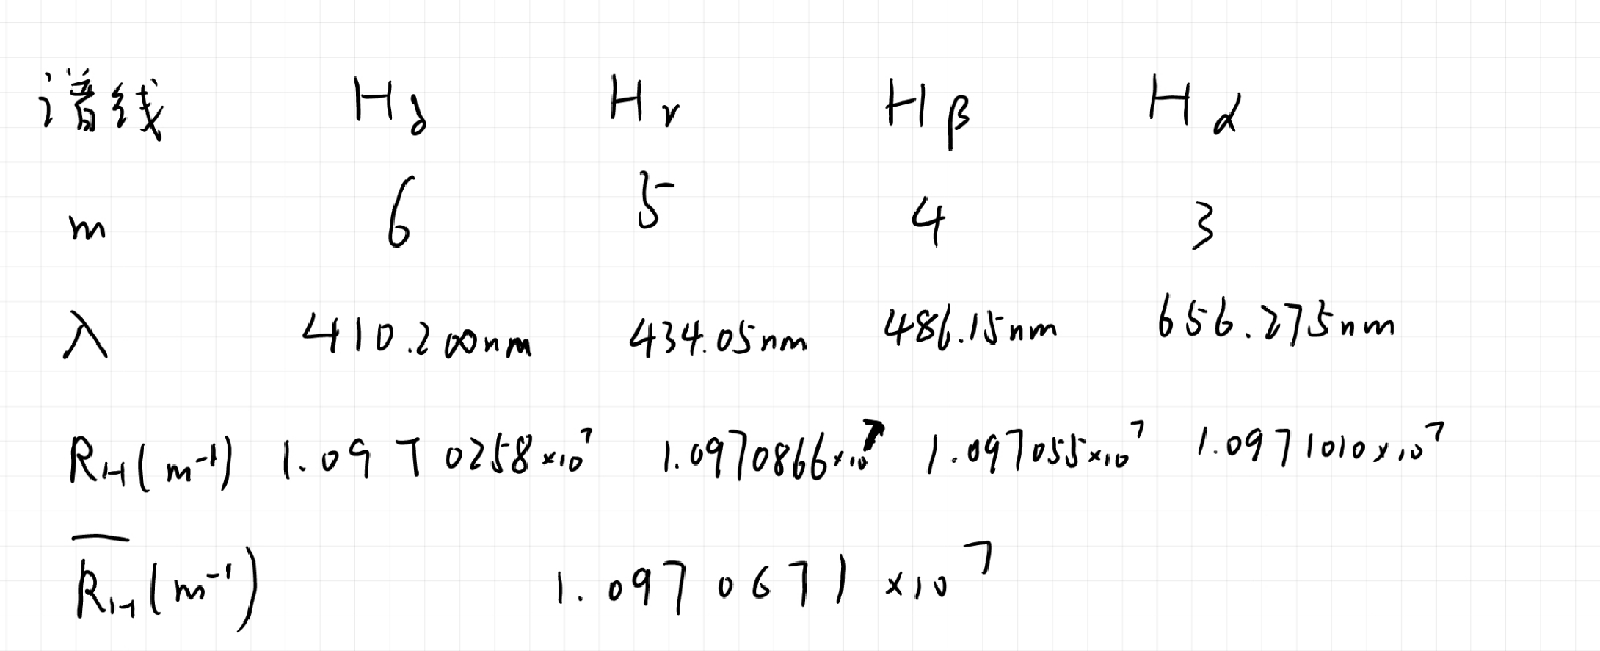
\includegraphics[width=1\textwidth]{1.jpg}
    \caption{\label{Lab12}实验数据处理}
    \end{figure}


\subsection*{测量汞灯的光谱曲线}
\begin{figure}[H]
    \centering
    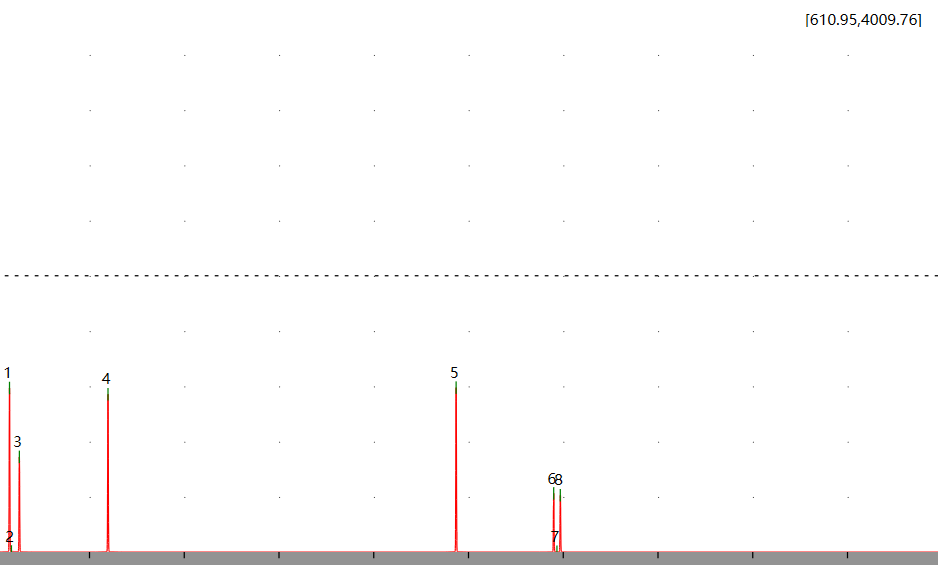
\includegraphics[width=1\textwidth]{虚拟1/汞灯1.png}
    \caption{\label{Lab12}汞灯}
    \end{figure}

    \begin{figure}[H]
        \centering
        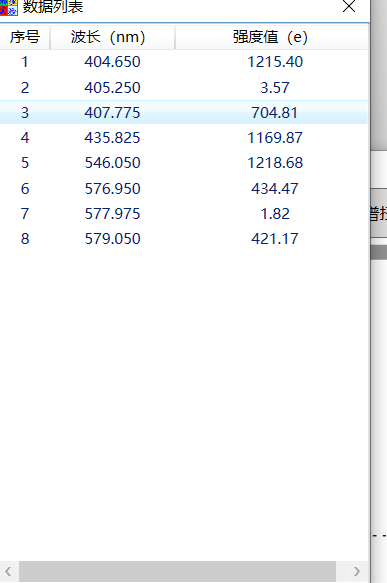
\includegraphics[width=0.5\textwidth]{虚拟1/汞灯2.png}
        \caption{\label{Lab12}汞灯}
        \end{figure}


\section*{四、总结与分析}

\subsection*{思考题}

\subsubsection*{1.解释光栅单色仪的原理}

单色仪是一种分光仪器,它通过色散元件的分光作用,把复色光分解成它的单色组成。

平面光栅单色仪的工作原理是光源发出的光均匀地照亮在入射狭缝S1上,S1位于离轴抛物镜的焦面上。光经过M1平行照射到光栅上,并经过光栅的衍射回到M1,经M1反射的光经过M2会聚到S2出射狭缝上。由于光栅的衍射作用,从出射狭缝出来的光线为单色光。当光栅转动时,从出射狭缝里出来的光由短波到长波依次出现。

\subsubsection*{为什么光栅的衍射图样会比单缝衍射或双缝衍射呈现的条纹更细更亮?}
在光栅衍射中,由于狭缝数目的增加,对新的衍射光强进行分析可以看出,峰值周边的值会下降很多,因此会有分辨率的提升,当N越大时,分辨率越高,得到的条纹就更细更亮.


衍射光栅在屏幕上产生的光谱线的位置,可用式$(a+b)(sin\phi+/-sin\theta = k\lambda)$表示。式中a代表狭缝宽度,b代表狭缝间距,φ为衍射角,θ为光的入射方向与光栅平面法线之间的夹角,k为明条纹光谱级数(k=0,±1,±2……),λ为波长,a+b称作光栅常数。用此式可以计算光波波长。光栅产生的条纹的特点是:明条纹很亮很窄,相邻明纹间的暗区很宽,衍射图样十分清晰。因而利用光栅衍射可以精确地测定波长。衍射光栅的分辨本领R=l/Dl=kN。其中N为狭缝数,狭缝数越多明条纹越亮、越细,光栅分辨本领就越高。

\subsection*{实验总结}
本次线上实验,光栅单色仪的方法我测量了氢原子和汞灯的特征谱线,并且通过对氢原子光谱的分析计算得到了里德堡常数,
线上的光学实验相比于线上的操作更为简单,对其背后的物理原理能有一个直观的感受,实验的整体操作和处理都是十分容易的.

\end{document}